\section{Zielsetzung}

In diesem Versuch sollen die Suszeptibilitäten verschiedener paramagnetischer Seltener-Erde-Verbindungen untersucht werden.

\section{Theorie}
\label{sec:Theorie}

In Materie setzt sich die magnetische Flussdichte $\vec{B}$ sowohl aus der magnetischen Feldstärke $\vec{H}$, wie auch der Magnetisierung $\vec{M}$ zusammen.
Dabei gilt die Relation 

\begin{equation}
    \label{eqn:mag-allg}
    \vec{B} = \mu_0 \vec{H} + \vec{M},
\end{equation}

wobei $\mu_0$ die magnetische Feldkonstante. 
Die Magnetisierung wird durch die magnetischen Momente in der Materie hervorgerufen und hängt nach 

\begin{equation}
    \label{eqn:magnetisierung}
    \vec{M} = \mu_0 \chi \vec{H}
\end{equation}

ebenfalls von der Feldstärke ab.
Dabei ist $\chi$ die sogenannte magnetische Suszeptibilität. Diese hängt sowohl von dem Material, von $\vec{H}$, als auch von der Temperatur $T$ ab.
Diese sorgt für Änderungenen in der Orientierung der Dipolmomente im Material.

An dieser Stelle sei gesagt, dass der hier zu untersuchende Paramagnetismus, im Gegensatz zum Diamagnetismus, nicht bei jedem Material auftritt.
Dies liegt daran, dass ersterer nur zu finden ist, wenn die Atome im Material einen endlichen Drehimpuls besitzen.

Im einem Atom liegen einerseits die Spins der Elektronen $\vec{S}$ und deren Bahndrehimpulse $\vec{L}$ vor.
Dies setzt sich additiv zum Gesamtdrehimpuls $\vec{J}$ zusammen.
Damit sind die Dipolmomente durch

\begin{align}
    \vec{\mu_\text{L}} &= - \frac{\mu_\text{B}}{\hslash} \vec{L} \\
    \vec{\mu_\text{S}} &= - g_\text{S} \frac{\mu_\text{B}}{\hslash} \vec{S}
\end{align}

gegeben, wobei $\mu_\text{B}$ das Bohr'sche Magneton und $g_\text{S}$ das gyromagnetische Verhältnis ist.

\begin{figure}
    \centering
    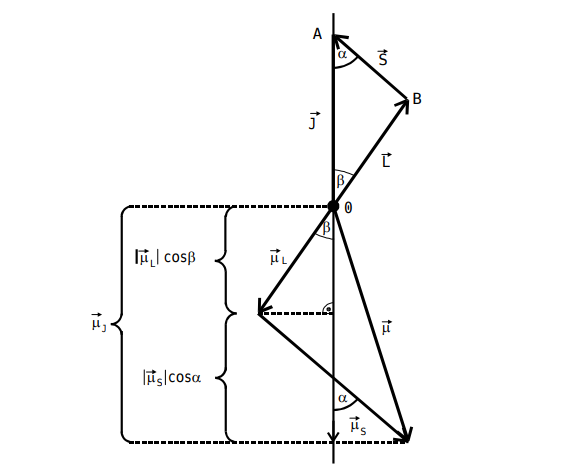
\includegraphics{skizze-drehimpuls.png}
    \caption{Skizze zur Vektoraddition der Drehimpulse und der magnetischen Momente im Atom \cite{V606}.}
    \label{fig:skizze-dreh}
\end{figure}

Des Weiteren liefert die Quantenmechanik für die Beträge von $\vec{L}$, $\{vec{S}$ und $\vec{J}$ die Relationen

\begin{align} 
    |\vec{L}| = L &= \sqrt{ L ( L + 1 ) } \hslash \\
    |\vec{S}| = S &= \sqrt{ S ( S + 1 ) } \hslash \\
    |\vec{J}| = J &= \sqrt{ J ( J + 1 ) } \hslash.
\end{align}

Mit den Winkelbeziehungen in \autoref{fig:skizze-dreh} und der Näherung $g_\text{S} = 2$ lässt sich das magnetische Moment zum Gesamtdrehimpuls als

\begin{equation}
    \label{eqn:magn-moment}
    \mu_\text{J} = g_\text{J} \cdot \mu_\text{B} \sqrt{J (J + 1)}
\end{equation}

schreiben, wobei 

\begin{equation}
    \label{eqn:lande}
    g_\text{J} := \frac{ 3 J (J+1) + S(S+1) - L(L+1) }{ 2 J (J +1) }
\end{equation}

der Landé-Faktor ist.